\documentclass[a4paper,10pt]{article}
\usepackage[utf8]{inputenc}
\usepackage[margin=0.5in]{geometry}
\usepackage{amsmath}
\usepackage{xfrac}
\usepackage{listings}
\usepackage{graphicx}
\usepackage{wrapfig}
\usepackage{adjustbox}
\graphicspath{{figures/}}


%opening
\title{JAnalysisTools Manual}
\author{J. T. Smallcombe}
\begin{document}

\maketitle
\tableofcontents

\section{Introduction}
This library designed to help working with root for analysis contains several GUI analysis tools and useful sets of functions. An explanation of some of the major components is given here, but subclasses and functions will not be detailed.
Various histogram presentation formating and automated fitting macros (for spectroscopic peaks and detector efficiency curves) are also included and may be documented later. 

\section{Install}
This library has only been tested with ROOT6, it does not currently have any other non-standard dependencies.
Source the ROOT6 $thisroot.sh$.
In the base directory of the library run:
\lstset{language=bash}
\begin{lstlisting}
make clean
make -j 4
source bin/thisjlib.sh
root -l bin/root_start.C
\end{lstlisting}
If all worked well root started without error messages and is running with the library loaded.
For future use add a source of $thisjlib.sh$ to your bashrc and add $gSystem->Load("libJanalysistools.so")$ to your root startup script.

\section{jEnv Toolbar}
A graphical session manager toolbar to handle grabbing (selecting) of histograms with no typing.
To create a new instance simply type:
\lstset{language=C++}
\begin{lstlisting}
new jEnv();
\end{lstlisting}
in a ROOT interactive session. A new window will open:
\renewcommand{\labelenumi}{\Alph{enumi}}
\begin{center}
\begin{tabular}{ c c }
\begin{minipage}{0.7\textwidth}
\begin{enumerate}
\item Grabbed Histogram Icon
\item Open a new peak fitting environment (copy grabbed histogram if $TH1$)
\item Open a new 2/3D gating tool if grabbed histogram is $TH2/TH3$.
\item Open a new TBrowser and draw grabbed.
\item Create a new canvas and draw a copy of grabbed
\item Open a dialogue box to save grabbed to disk
\item Close the toolbar.
\item Exit root
\item Open/Close the AddSub Tool panel.
\end{enumerate} \end{minipage}
&
\raisebox{-.5\height}{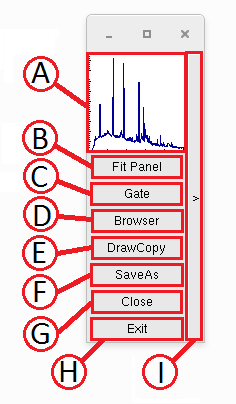
\includegraphics[width=0.23\textwidth]{jEnvA.png}}
\\
\end{tabular}
\end{center}

%\begin{wrapfigure}{r}{0.25\textwidth}
%\end{wrapfigure}
\subsection{Histogram Grabbing}
Whenever an instance of jEnv exists histogram grabbing is enabled in all $TCanvas$s, including those embedded in other classes/windows. Whenever a window containing a drawn histogram is clicked, a pointer to the first histogram of the frame is grabbed by jEnv and the small "Selected Histogram" icon will change. If a frame contains multiple histograms and you must click exactly on the desired histogram itself, not on the whitespace.

\begin{figure*}[!h]
\centering
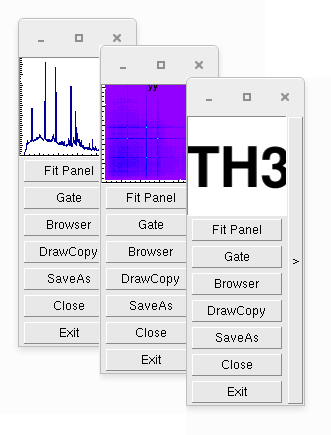
\includegraphics[width=0.3\textwidth]{jEnvB.png}
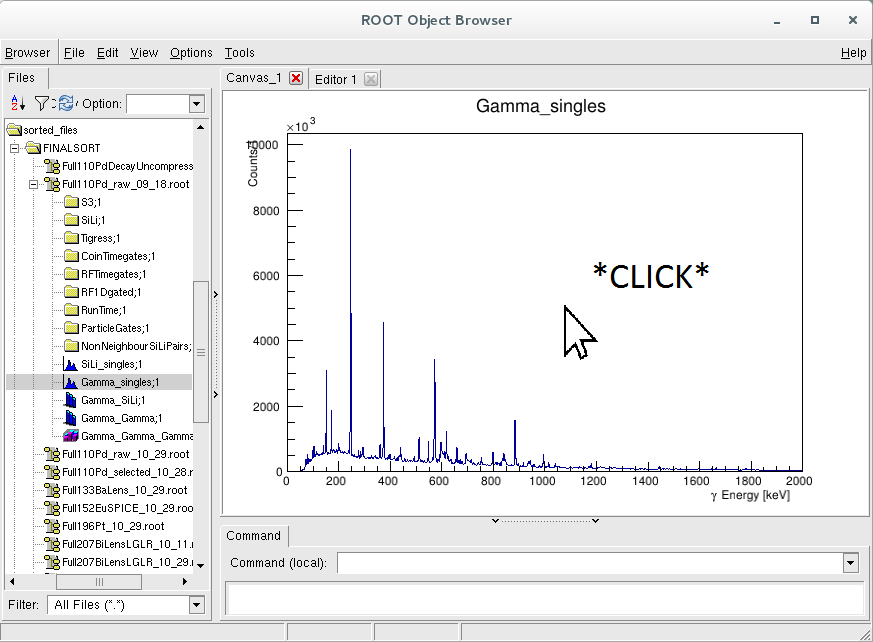
\includegraphics[width=0.52\textwidth]{jEnvD.png}     
\end{figure*}

Once a histogram is grabbed a copy of it will be passed to any of the functions of jEnv.

\subsubsection{Histogram Lifetime}
A histogram can go out of memory scope in several ways. For speed, as grabbing is done on EVERY canvas click, only a pointer is stored. jEnv will refuse to do anything with its histogram pointer until it has established it is valid. To check if a histogram is still in memory jEnv checks the histogram against roots list of object, however this object search has limitations. If this histogram is still drawn in the same canvas as when it was grabbed, it will be found.

\subsection{Histogram AddSub Tool}
Hidden in the side of jEnv is the AddSub tool. This is a simple tool to allow quick addition and subtraction of $TH1$s from anywhere. The tool even allows histograms with different binning, summing is done based on "user coordinates".
Click either of the selected histograms windows $A$ or $B$ to assign the currently grabbed histogram from jEnv, at this point a copy IS saved. The projected histogram is then given by $A\pm B*f$ where f is the fraction specified by the slider. In the case of subtraction the area of B is first normalised to that of A. The resultant histogram can also be grabbed.

\begin{center}
\begin{tabular}{ c c }
\begin{minipage}{0.4\textwidth}
\begin{enumerate}
\item Open/Close the AddSub Tool panel.
\item Subtraction/Addition fraction $f$ slider.
\item Selected Histogram A window/button
\item Swap A B
\item Selected Histogram B window/button
\item Fraction $f$ text entry.
\item Change between Subtraction/Addition.
\item Hide/Show error bars when drawing.
\item Result Window.
\end{enumerate} \end{minipage}
&
\raisebox{-.5\height}{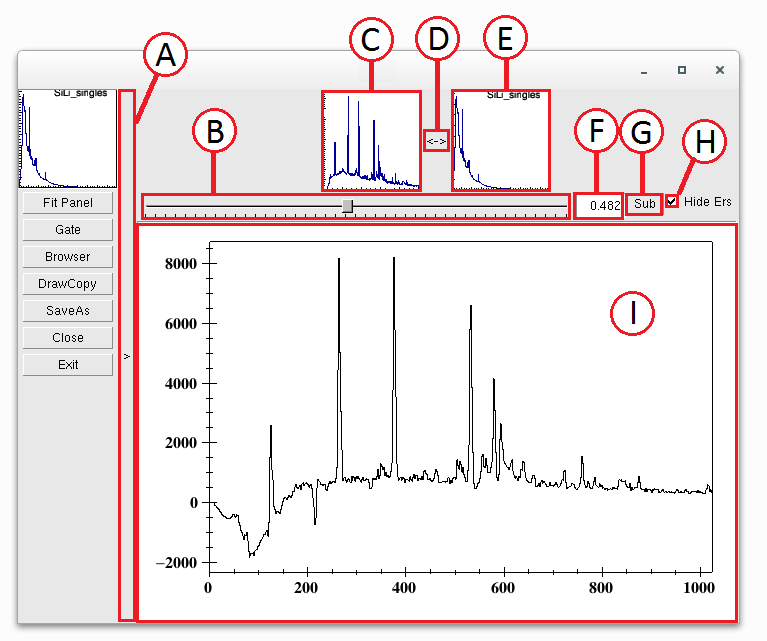
\includegraphics[width=0.55\textwidth]{jEnvC.png}}
\\
\end{tabular}
\end{center}

\section{Gating and Background Subtraction Tool}
The gating tool is designed to provide live graphical gating and background subtraction for $TH2$ and $TH3$ histograms filled with any data. 
A new instance can be created from the jEnv toolbar or typing any of the following:
\lstset{language=C++}
\begin{lstlisting}
new jEnv();
new jgating_tool();
new jgating_tool(TH2*/TH3*);
new jgating_tool(HistogramName);
\end{lstlisting}
where "HistogramName" is the name (not title) of a histogram open in memory. The call with no arguments will grab the most recently selected or drawn histogram. If no valid input is found a window will not appear. Please wait a moment for the window to appear when using $TH3$s, particularly if they are large.

\subsection{2D Gating Window}

1. Show the "with overflow" projection
2. Hide the Peak Fit Centroid tooltip.
3. Select the axis on which to gate (USE TO RESET IF ERRORS)
4. Background subtraction type


The fitting tool is "connected" to the result canvas and will connect with new input if the gate is changed. (see section ...)

\subsection{3D Gating Window}

For the first gate on a $TH3$ there is significant amount of computation so this is not done live. The output of the first gate is only performed when a new projection is selected, a different background mode is selected or when the [Update] button is pressed.

\subsection{Gate Summing Tool}





\section{Peak Fitting Tool}
The tool has some foibles that are absent from the root fitting environment, but it is far more tuned to the task of fitting spectra and saving the relevant data.

The fitting tool stores an internal copy of the histogram to avoid empty fitting segfaults.

The fitting tool is "connected" to the selected canvas, not to a particular histogram. When a new histogram is drawn in the canvas the fitting tool updates it's internal histogram accordingly. Note, you cannot modify a histogram through the canvas the fitting tool is connected to (as the fitting tool performs $DrawCopy$ of it's internal histogram).

\section{Histogram Formatting Functions}

\end{document}
